%%%%%%%%%%%%%%%%%%%%%%%%%%%%%%%%%%%%%%%%%
% Beamer Presentation
% LaTeX Template
% Version 1.0 (10/11/12)
%
% This template has been downloaded from:
% http://www.LaTeXTemplates.com
%
% License:
% CC BY-NC-SA 3.0 (http://creativecommons.org/licenses/by-nc-sa/3.0/)
%
%%%%%%%%%%%%%%%%%%%%%%%%%%%%%%%%%%%%%%%%%

%----------------------------------------------------------------------------------------
%	PACKAGES AND THEMES
%----------------------------------------------------------------------------------------

\documentclass{beamer}

\mode<presentation> {

% The Beamer class comes with a number of default slide themes
% which change the colors and layouts of slides. Below this is a list
% of all the themes, uncomment each in turn to see what they look like.

%\usetheme{default}
%\usetheme{AnnArbor}
%\usetheme{Antibes}
%\usetheme{Bergen}
%\usetheme{Berkeley}
%\usetheme{Berlin}
%\usetheme{Boadilla}
%\usetheme{CambridgeUS}
%\usetheme{Copenhagen}
%\usetheme{Darmstadt}
%\usetheme{Dresden}
%\usetheme{Frankfurt}
%\usetheme{Goettingen}
%\usetheme{Hannover}
%\usetheme{Ilmenau}
%\usetheme{JuanLesPins}
%\usetheme{Luebeck}
\usetheme{Madrid}
%\usetheme{Malmoe}
%\usetheme{Marburg}
%\usetheme{Montpellier}
%\usetheme{PaloAlto}
%\usetheme{Pittsburgh}
%\usetheme{Rochester}
%\usetheme{Singapore}
%\usetheme{Szeged}
%\usetheme{Warsaw}

% As well as themes, the Beamer class has a number of color themes
% for any slide theme. Uncomment each of these in turn to see how it
% changes the colors of your current slide theme.

%\usecolortheme{albatross}
%\usecolortheme{beaver}
%\usecolortheme{beetle}
%\usecolortheme{crane}
%\usecolortheme{dolphin}
%\usecolortheme{dove}
%\usecolortheme{fly}
%\usecolortheme{lily}
%\usecolortheme{orchid}
%\usecolortheme{rose}
%\usecolortheme{seagull}
\usecolortheme{seahorse}
%\usecolortheme{whale}
%\usecolortheme{wolverine}

%\setbeamertemplate{footline} % To remove the footer line in all slides uncomment this line
%\setbeamertemplate{footline}[page number] % To replace the footer line in all slides with a simple slide count uncomment this line

%\setbeamertemplate{navigation symbols}{} % To remove the navigation symbols from the bottom of all slides uncomment this line
}

\usepackage{graphicx} % Allows including images
\usepackage{booktabs} % Allows the use of \toprule, \midrule and \bottomrule in tables
\usepackage[utf8]{inputenc}
\usepackage[spanish]{babel}
\decimalpoint
%\usecolortheme[rgb={0.6,0.3,0.2}]{structure} % para setear color
%----------------------------------------------------------------------------------------
%	TITLE PAGE
%----------------------------------------------------------------------------------------

\title[Propuesta de Tesis De Magíster]{Ensamble de Modelos Sintácticos y Semánticos para la Evaluación Automática de Ensayos} % The short title appears at the bottom of every slide, the full title is only on the title page

\author{Diego Palma S.} % Your name
\institute[UDEC] % Your institution as it will appear on the bottom of every slide, may be shorthand to save space
{
Profesor Supervisor: John Atkinson \\
\medskip
Universidad de Concepción \\ % Your institution for the title page
\medskip
\textit{dipalma@udec.cl} % Your email address
}
\date{\today} % Date, can be changed to a custom date

\begin{document}

\begin{frame}
\titlepage % Print the title page as the first slide
\end{frame}

\begin{frame}
\frametitle{Contenido} % Table of contents slide, comment this block out to remove it
\tableofcontents % Throughout your presentation, if you choose to use \section{} and \subsection{} commands, these will automatically be printed on this slide as an overview of your presentation
\end{frame}

%----------------------------------------------------------------------------------------
%	PRESENTATION SLIDES
%----------------------------------------------------------------------------------------

%------------------------------------------------
\section{Introducción} % Sections can be created in order to organize your presentation into discrete blocks, all sections and subsections are automatically printed in the table of contents as an overview of the talk
%------------------------------------------------

\begin{frame}
\frametitle{Introducción}
\begin{itemize}
\item Hoy en día los sistemas de recomendación son una componente importante en el comercio electrónico.
\item Estos sistemas, buscan recomendar ciertos ítemes a un usuario en base a su perfil. El perfil de usuario se intenta inferir de acuerdo a su historial de compras, y preferencias.
\item A pesar del amplio uso de estos sistemas de recomendación, el no considerar la situación actual del usuario podría resultar en malas recomendaciones. (Ej: Comprar un juguete para un sobrino, etc.)
\item Para solucionar este problema, se introduce la noción de contexto y los sistemas de recomendación que consideran contexto ({\em Context-Aware Recommender Systems} CARS)
\end{itemize}
\end{frame}

%------------------------------------------------

\begin{frame}
\frametitle{Introducción}
\begin{block}{Hipótesis}
Un método de evaluación de textos que considere características sintácticas y semánticas para evaluar coherencia textual será más efectivo para la tarea de evaluación automática de ensayos en comparación métodos que utilicen medidas superficiales estadísticas.
\end{block}

\end{frame}

\begin{frame}
\begin{block}{Objetivos}
\begin{itemize}
	\item Objetivo General
	\begin{itemize}
		\item Desarrollar un método computacional que permita evaluar automáticamente textos en forma de ensayos considerando aspectos de coherencia textual.
	\end{itemize}
	\item Objetivos Específicos
	\begin{itemize}
		\item Analizar estrategias de evaluación de ensayos en forma de texto, basados tanto en modelos de estadísticos, como en teoría de discurso.
		\item Desarrollar una estrategia que considere coherencia a nivel de contenido y sintaxis.
		\item Crear un prototipo para realizar las pruebas.
		\item Evaluar el modelo propuesto.
	\end{itemize}
\end{itemize}
\end{block}
\end{frame}
%------------------------------------------------

\section{Trabajo Relacionado}
\begin{frame}
\frametitle{Trabajo Relacionado}
Métodos basados en características superficiales:

\begin{itemize}
\item Representan los textos como un conjunto de características que se utilizan como medidas indirectas de propiedades del texto tales como: Coherencia, cohesión, contenido.
\item La nota se calcula como una suma ponderada de estas características (generalmente se utiliza regresión). El primer sistema exitoso (PEG) utilizaba regresión lineal.
\item Para obtener la ponderación de cada característica, se requiere tener un conjunto de ensayos previamente evaluados.
\begin{block}{Similaridad Contextual}
\begin{equation}
	Nota = \beta_0 + \sum_{i=1}^n \beta_i P_i
\end{equation}
\end{block}


\end{itemize}

\end{frame}

%------------------------------------------------

\begingroup
\small
\begin{frame}
\frametitle{Trabajo Relacionado}
Modelo de Espacio Vectorial

\begin{figure}
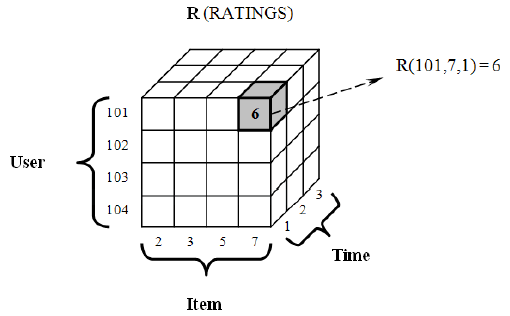
\includegraphics[width=0.5\linewidth]{user_item_context.png}
\end{figure}

\begin{itemize}
\item Los sistemas de recomendación descritos previamente sólo utilizan información básica del usuario y del ítem.
\item Se agrega el ``contexto'', que podría ser una época del año (ejemplo: Recomendaciones de lugares para viajar en invierno y verano).
\item El contexto y sus atributos dependerá del dominio en particular (ejemplo: música y estado anímico).
\end{itemize}

\end{frame}
\endgroup

%------------------------------------------------

\begin{frame}
\frametitle{Trabajo Relacionado}
\begin{itemize}
\item En general el contexto puede ser explícito, implícito o puede ser inferido.
\item En el caso explícito, se obtiene información directa del usuario, por ejemplo mediante cuestionarios, o preferencias. (Problema: Se requiere participación directa del usuario)
\item En el caso implícito, el contexto puede obtenerse detectando ``cambios'' en el usuario, por ejemplo cambios en su ubicación (GPS), o fechas de últimas transacciones. (Problema: No siempre se obtiene información relevante)
\item Se puede inferir el contexto aplicando técnicas de minado de datos. Se requiere construir un modelo predictivo (por ejemplo un clasificador).
\end{itemize}

\end{frame}

%------------------------------------------------

\section{Método Propuesto}
\begin{frame}
\frametitle{Método Propuesto}
\begin{itemize}
\item El método propuesto se utiliza en el dominio de recomendaciones para viajes.
\item Se extrae el contexto del usuario a partir de una consulta. Ejemplo:

\begin{figure}
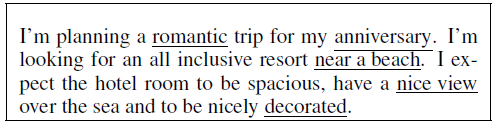
\includegraphics[width=0.5\linewidth]{query.png}
\end{figure}

\item Se hace el supuesto de que existen etiquetas explícitas que representan el contexto del usuario. En este dominio, el tipo de viaje.

\item El contexto se representa como una función de distribución sobre las etiquetas posibles que puede tener un viaje.

\end{itemize}

\end{frame}

%------------------------------------------------

\begin{frame}
\frametitle{Método Propuesto}
\begin{itemize}

\item No en todas las consultas estará explícito el contexto, por lo que se requiere un mecanismo de inferencia.

\item La información necesaria para realizar las inferencias se extrae de las reseñas dadas por distintos usuarios.

\item Por ejemplo, si en la reseña del usuario $u$ se indica el tipo de viaje para el hotel $i$ como ``business'' y ``Solo Travel'':

$Context_u^i = \{P(family) = 0, P(couples) = 0, P(solo \ travel) = 0.5, P(business) = 0.5, P(friend's \ get \ away) = 0\}$

\item El problema de inferencia descrito es similar al problema de clasificación de textos con varias etiquetas, en el cual, un texto puede ser clasificado en una o más categorías.

\end{itemize}
\end{frame}

%------------------------------------------------

\begin{frame}
\frametitle{Método Propuesto}
\begin{itemize}
\item Se escogió Labeled-LDA (L-LDA) como método de categorización de textos.
\item L-LDA es una extensión de LDA (Latent Dirichlet Allocation).
\item LDA representa los documentos en un CORPUS como una mezcla de K tópicos. En la fase de entrenamiento LDA ``aprende'' la representación de tópicos de cada documento y las palabras asociadas a cada tópico.
\end{itemize}

\end{frame}

%------------------------------------------------

\begin{frame}
\frametitle{Método Propuesto}
Ejemplo LDA
\begin{itemize}
\item Suponga que se tienen las siguientes oraciones:
\begin{enumerate}
\item I ate a banana and spinach smoothie for breakfast.
\item I like to eat broccoli and bananas.
\item Chinchillas and kittens are cute.
\item My sister adopted a kitten yesterday.
\item Look at this cute hamster munching on a piece of broccoli.
\end{enumerate}
\item Utilizando LDA y 2 tópicos:
\begin{itemize}
\item Oraciones 1 y 2: 100\% tópico A.
\item Oraciones 3 y 4: 100\% tópico B.
\item Oración 5: 60\% tópico A, 40\% tópico B.
\item Tópico A: 30\% broccoli, 15\% bannanas, 10\% breakfast, 10\% munching... (Se podría interpretar como un tópico que habla sobre comida)
\item Tópico B: 20\% chinchillas, 20\% kittens, 20\% cute, 15\% hamster... (Se podría interpretar el tópico como animales tiernos)
\end{itemize}
\end{itemize}
\end{frame}
%------------------------------------------------

\begin{frame}
\frametitle{Método Propuesto}
\begin{itemize}
\item LDA es un método no supervisado. L-LDA impone restricciones sobre LDA para clasificar documentos según tópicos previamente definidos.
\item Luego se puede clasificar una consulta dada, e ``inferir'' el contexto del usuario para realizar las recomendaciones.
\item Por otro lado, utilizando el historial de ``reviews'' de los usuarios, se puede predecir el contexto de un usuario:
\end{itemize}

\begin{block}{Similaridad Contextual}
$contextualSimilarity(i, j) = \displaystyle \frac{\sum_u commonLabels(i, j)}{\sqrt{\sum_u |labels(i)|x|labels(i)|}}$
\end{block}

\begin{block}{Predicción del contexto}
$predictedContext(u, i) = \displaystyle \frac{\sum_{k\in Neighbors(i)}context_u^k\cdot contextualSimilarity(k, i)}{\sum_{k\in Neighbors(i)} |contextualSimilarity(k, i)|}$
\end{block}

\end{frame}

\begin{frame}
Finalmente, utilizando el contexto previsto y el contexto inferido, se puede estimar cuánta utilidad le aporta el ítem al usuario:

\begin{block}{Puntaje Contextual}
$contextScore(u, i) = \displaystyle \frac{IC_u \cdot PC_u^i}{\|IC_u\|\|PC_u^i\|}$
\end{block}

\begin{block}{Utilidad}
$utility(u, i) = \alpha predictedRating(u, i) + (1 - \alpha) contextScore(u. i)$
\end{block}

Donde $predictedRating(u, i)$ se obtiene mediante métodos tradicionales (como filtrado colaborativo), y $\alpha$ es una constante que representa el peso del puntaje previsto para el item.
\end{frame}

%----------------------------------------------------------------------------------------

\section{Evaluación del método propuesto}

\begin{frame}
\frametitle{Evaluación del Método propuesto}

\begin{itemize}
\item Como no se está estimando la nota que el usuario le daría a un item en particular, no tiene sentido utilizar métricas como MAE u otras que comparan la nota estimada con la real.
\item Se propone utilizar la métrica Hit Ratio.
\item Se utilizó validación cruzada dejando uno fuera. Se calculó el {\em Hit Ratio} para dicho ítem.
\end{itemize}

\begin{block} {Hit Ratio}
$Hit \ Ratio_i = \sum_{u\in U_T} \displaystyle \frac{H_{ui}}{|U_T|}$
\end{block}

Donde $U_T$ son los usuarios en el conjunto de pruebas, $H_{ui} = 1$ el item $i$ es recomendado al usuario $u$ (0 en caso contrario). En palabras simples, el {\em hit ratio} es la probabilidad de que el ítem $i$ sea recomendado en $N$ conjuntos de recomendaciones.

\end{frame}

\begin{frame}
\frametitle{Evaluación del Método propuesto}

\begin{figure}
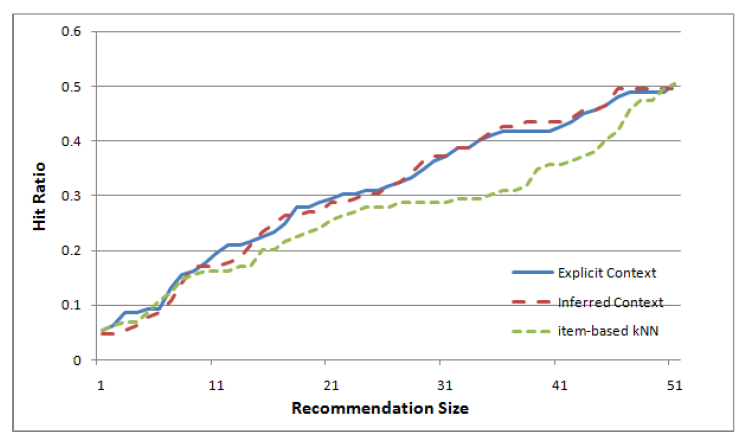
\includegraphics[width=0.7\linewidth]{evaluation.png}
\end{figure}

\end{frame}

%----------------------------------------------------------------------------------------

\section{Conclusiones}
\begin{frame}
\frametitle{Conclusiones}

\begin{itemize}
\item Se propuso un nuevo enfoque para el minado de contexto desde un texto en lenguaje natural, y se utilizó para producir recomendaciones que consideraran contexto.
\item Las evaluaciones indican que utilizar información contextual mejora las recomendaciones en términos del {\em hit ratio}.
\end{itemize}

\end{frame}

%----------------------------------------------------------------------------------------

\begin{frame}
\Huge{\centerline{The End}}
\end{frame}

%----------------------------------------------------------------------------------------

\end{document} 